\section{Motivating Examples}
\label{s:motivation}

A user may use a VCS for multiple purposes: software configuration management,
backup service, sharing service, etc.\HP{Any more possible usage?}
Among these purposes, the most important and well-known is software
configuration management. This section will start from the review of
\textred{XXX} real life scenarios, continue with discussions of how traditional
VCSs reacts with those scenarios, and then end up with a list of properties an
ideal solution is desired to have.

\subsection{Scenarios}

%\textred{Describe Case \#1, 2, 4 in design\_v2.txt}
%\textred{Explain why traditional VCS could not solve those scenarios}

% Scenario #2
We start by taking a look at the first example in the introduction section.
\HP{Check if this is still consistent in final submission.}
In that example, a project manager wants a developer only able to view a part of
the whole project files. If the project is not version controlled and stored in
regular file systems, the project manager can restrict the permission of anyone
by assigning correct permissions in file systems. For example, in a \unix-like
file system, the project manager can restrict the \emph{read} permission to a user
by not adding that user to the \emph{group owner} of the file and assign no
\emph{global read permission} to the file.

% Scenario #1
A similar but different scenario is that a project manager wants to restrict a
developer only able to view a part of the \emph{commit history}. This happens
when some retro versions in the repository contains some commercial secrets that
should not be revealed to a new employee.

% Some discussions
Although both features are inherited in some old VCSs like CVS\cite{cvs}, it cannot
be done in most popular VCS today like \git\cite{git} and
\mercurial\cite{mercurial}. One of the reason is that \git and \mercurial use distributed data
model, which require the user to \emph{clone} the repository before any actual
work. When a user clone a repository, he or she must be able to \emph{read}
everything in it in order to copy it out. So the user is already able to view
any files in the repository. Therefore it makes no sense to further restrict
\emph{read} access to any user who have cloned the repository. As a result,
those VCS controls \emph{read} permission on an all-or-nothing basis: a user
either can access the whole repository, or nothing at all.

\iffalse
% HW: Inappropriate claim
%Another reason is that is a commit-based\HP{good word?} VCS, 
\fi

\begin{figure}[t]
\centerline{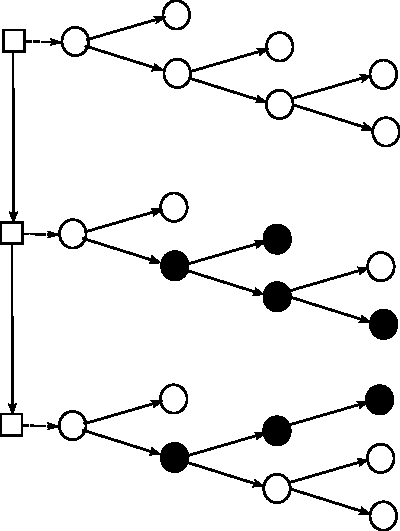
\includegraphics{fig/committree.pdf}}
\caption{A sample commit tree. In the graph, squares represent commit objects,
circles represent files or directories. The circles in black are allowed to
be accessed by a specific user.}
\label{f:commit-tree}
\end{figure}

\endinput




% Summarize the first two examples
These two examples could be considered as an integrity. The problem resided
behind the two examples is to restrict the access permissions in both time and
space. We can consider the commit history as a 2-dimensional, as depicted
in Figure \ref{f:commit-tree}.

\hw{TODO Scenario #4 and discussions}


\subsection{Properties}

\hw{Summarize the principles \sys is desired to have in order to solve those
scenarios.}

